\section{Introduction}
\label{sec:intro}

\subsection{The contest}
\label{sec:contest}

The Monarch of the Hill contest is a one-on-one match between autonomous robots on a hill of two \qty{5}{ft} (\qty{1.524}{m}) ramps that meet at a flat mesa \qty{33}{in} above the floor (Fig.~\ref{fig:hill}). The ramps are covered with a non-slip surface like a bathtub mat, and their angle is
\begin{equation}
  \sin\theta = \frac{\qty{33}{in}}{\qty{60}{in}} = 0.550, \qquad \theta = \ang{33.4}
  \label{eq:theta}
\end{equation}
Each robot starts on the slope at the bottom of its ramp, and a judge starts it with a single switch on the robot. After \qty{30}{s}, the robot whose farthest point is closest, in three dimensions, to the center of the mesa wins; a robot still on the hill beats one that has fallen off. The rules cap the robot at \qty{1}{kg}, require it to fit inside a \qty{1}{ft} cube at the start, forbid any remote control, and limit stored energy to the supplied two-cell (2S) 18650 lithium-ion pack plus small springs. Groups play 5 to 6 rounds in a Swiss-system tournament~\cite{ronney}.

\begin{figure}[htbp]
  \centering
  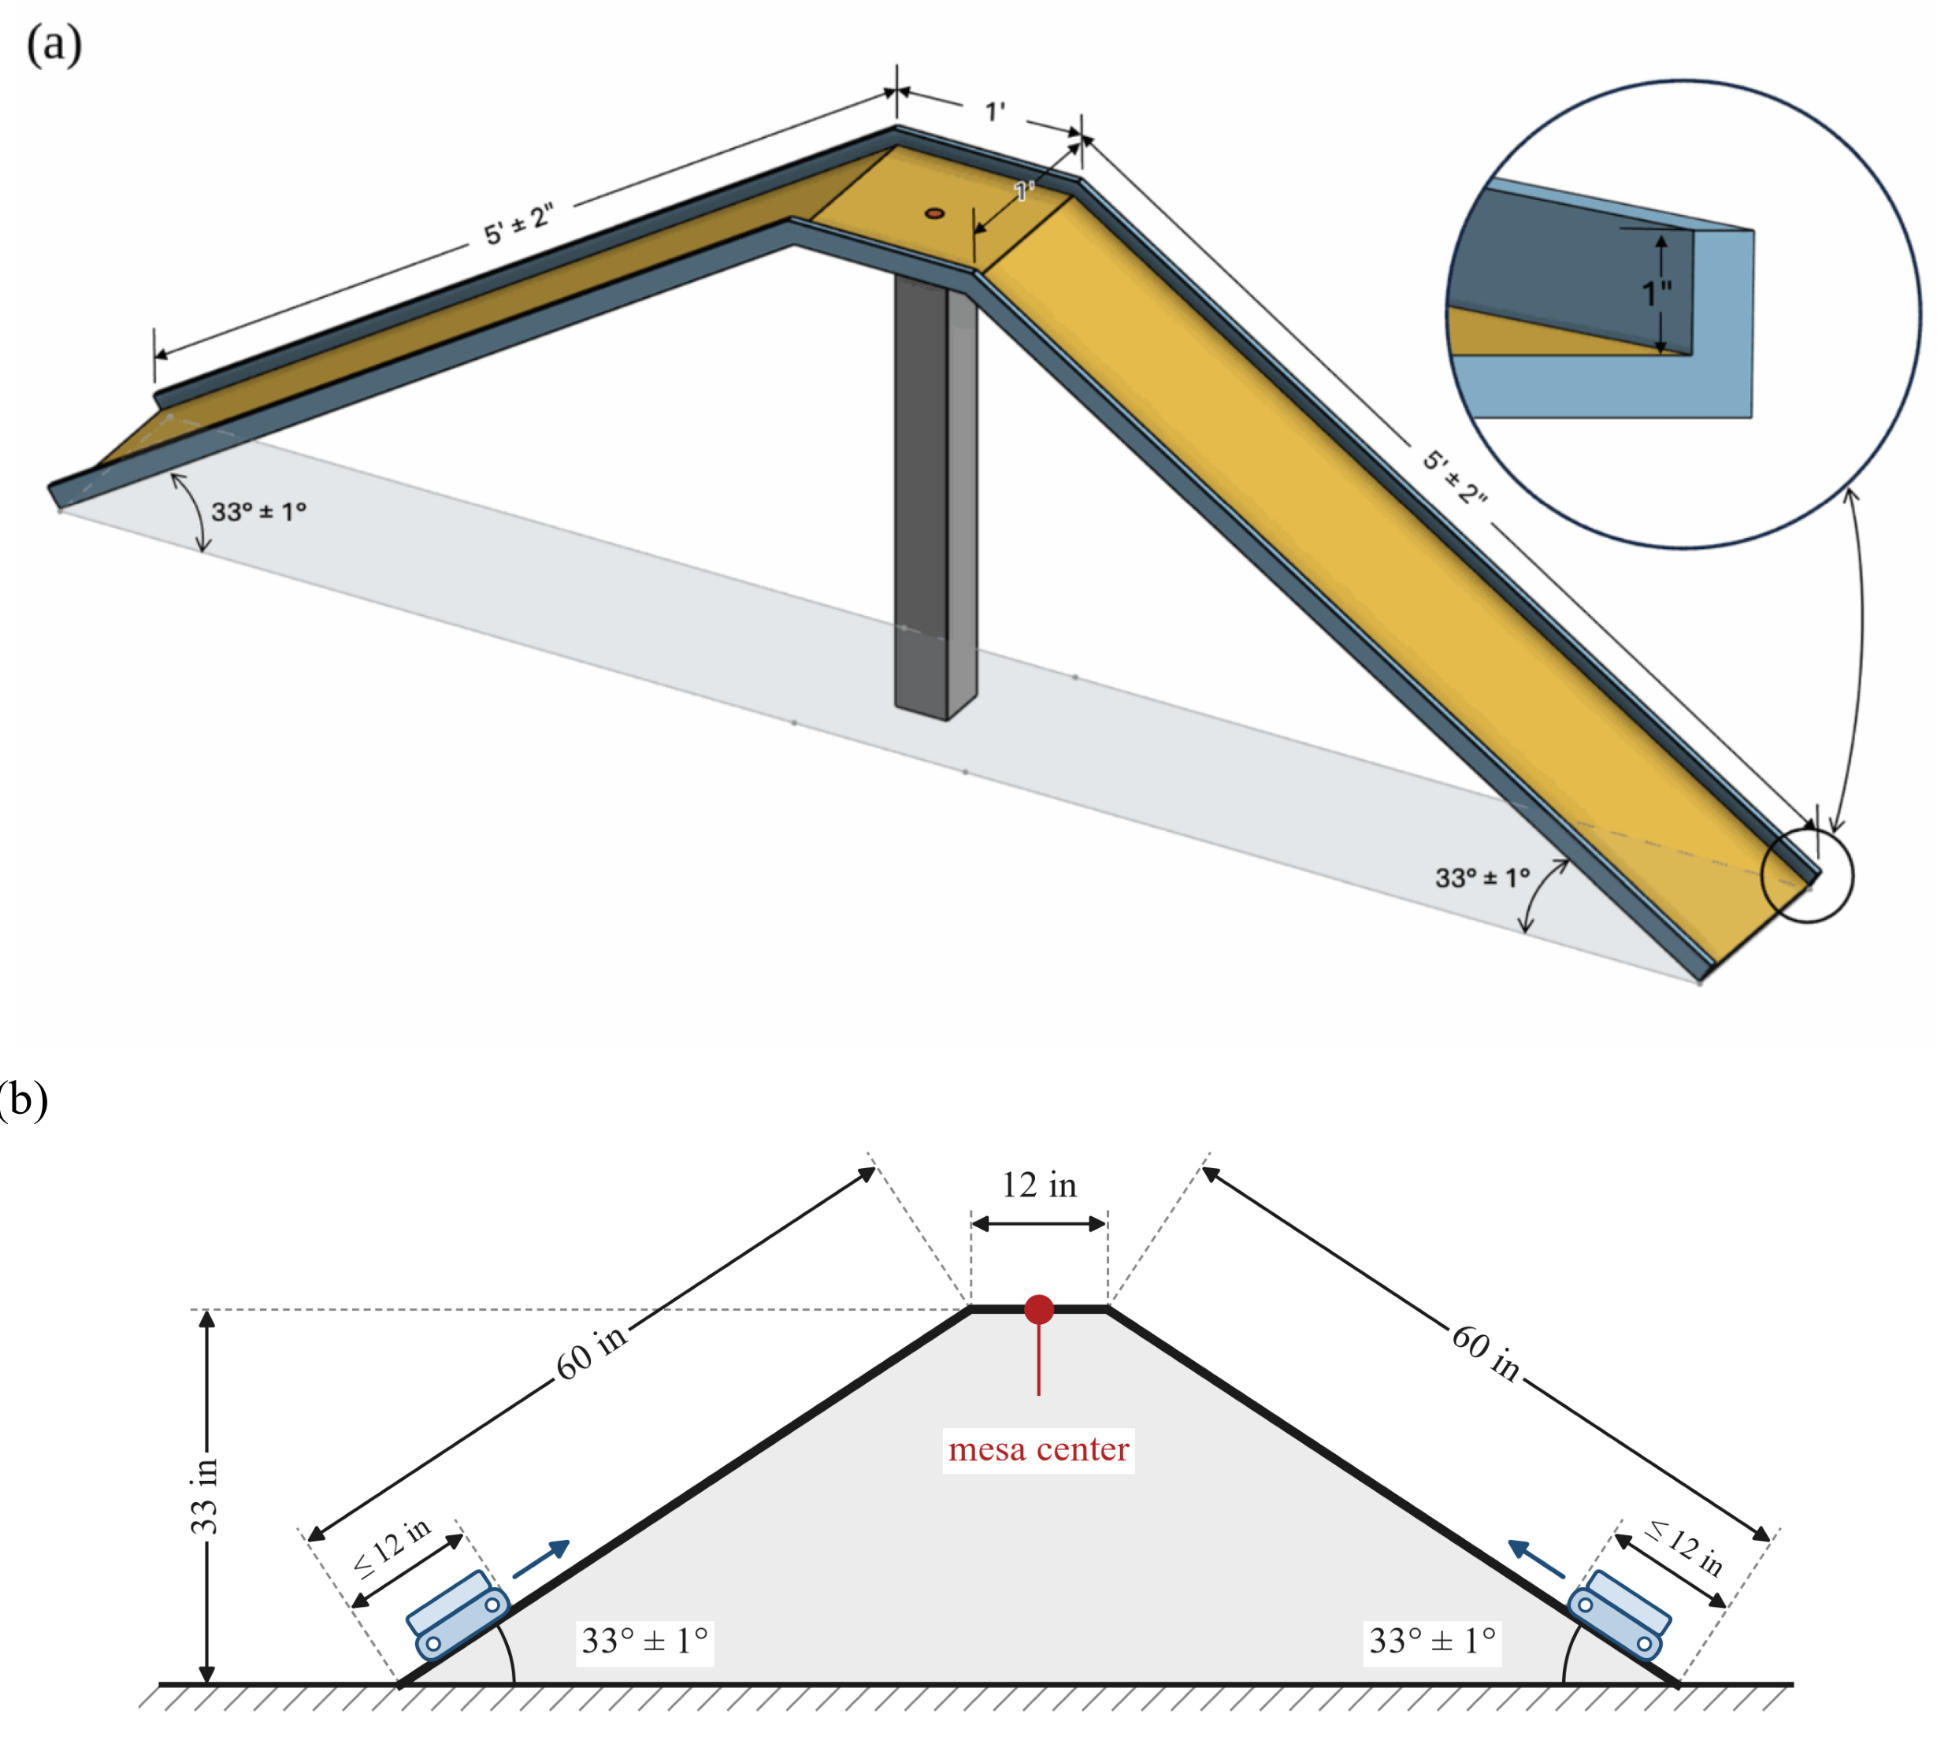
\includegraphics[width=0.85\textwidth]{fig01_hill.png}
  \caption{The contest hill. (a) Drawing from the course notes~\cite{ronney}. (b) Side view, to scale, with a robot on each ramp inside the \qty{12}{in} start zone.}
  \label{fig:hill}
\end{figure}

\subsection{Objective and strategy}
\label{sec:strategy}

Our objective was to reach the mesa first and keep the opponent from displacing us for the rest of the \qty{30}{s}. The lecture notes put it as ``possession is 9/10 of the law''~\cite{ronney}. The hill's geometry makes this even stronger. An attacker is still on the slope, fighting gravity, while the defender sits on the flat. And an attacker's wedge cannot sit flush until the robot has fully cleared the ramp, so its edge is still in the air at the moment it meets the defender.

Arriving first matters even more for an autonomous robot than for a driven one. Until the robots meet, the world is fully known: a \ang{33.4} slope of known length, then a flat mesa. After contact, a robot without vision cannot tell whether it is being pushed, lifted or turned, and ultrasonic range sensors are easy to confuse. A robot that is already on top needs very little information to hold its place.

The physics favors the defender too. On the flat mesa a robot can resist with its whole friction force, $\mu_s m g$. An attacker still on the ramp spends most of its traction holding itself on the slope and has only $\mu_s m g \cos\theta - m g \sin\theta$ left to push with. For two robots of equal mass and any $\mu_s$ between 0.8 and 1.0, the defender can resist 3.5 to 7 times the force the attacker can apply.

\paragraph{Defense without a pushing match}
Instead of planning to out-push an opponent, we put a low wedge with forks at the front of the robot, so an opponent arriving at the mesa edge drives up onto it and over or off the side. The forks are shaped to sit flush on the mesa even while the rest of the robot is still clearing the ramp (Section~\ref{sec:wedge}), so we never arrive with a raised edge ourselves. The stock kit robots have a flat polycarbonate bottom about 2 to \qty{3}{in} off the ground, which a low wedge slides under easily. \tbd{Confirm how sitting under an opponent scores under the farthest-point rule; our final match (Section~\ref{sec:results}) shows it can lose.}

\paragraph{The side wall as a guide rail}
The whole contest is a straight line, so the robot never has to turn. It does have to stay aligned: run straight up the ramp, not ride over the edge, and not waste energy scrubbing sideways. Running with one side against a guide rail does this mechanically, and side guards keep the robot from riding up over the rail (Section~\ref{sec:layout}).

These goals set four requirements that organize the rest of the report: climb as fast as traction and power allow, recognize the crest and stop at the front of the mesa, hold position there, and never depend on winning a sustained pushing match.
